\documentclass{article}
\usepackage[utf8]{inputenc}
\usepackage[english]{babel}
\usepackage{amsthm}
\usepackage{url}

\usepackage[margin=1in]{geometry}
\usepackage{float}
\usepackage{tcolorbox}
\usepackage{tocloft}
\usepackage{comment}
\usepackage[american]{circuitikz}
\usepackage{tikz}
\usepackage{framed}
\usepackage{tabulary}
\usepackage{graphics}
\usepackage{colortbl}
\usetikzlibrary{decorations.pathreplacing}

 
\newtheorem{theorem}{Theorem}[section]
\newtheorem{corollary}{Corollary}[theorem]
\newtheorem{lemma}[theorem]{Lemma}

\definecolor[named]{myLayoutColorAux}{RGB}{174,49,54}
\definecolor[named]{myLayoutColorMain}{RGB}{0,26,153}
\usepackage{color}
\definecolor{LightCyan}{rgb}{0.88,1,1}

\renewcommand{\cfttoctitlefont}{\color{myLayoutColorMain} \bfseries\Large}
\renewcommand{\cftloftitlefont}{\color{myLayoutColorMain} \bfseries\Large}

\setcounter{section}{-1}

\usepackage{xcolor}
\usepackage{listings}
\definecolor{vgreen}{RGB}{104,180,104}
\definecolor{vblue}{RGB}{49,49,255}
\definecolor{vorange}{RGB}{255,143,102}

\lstdefinestyle{verilog-style}
{
    language=Verilog,
    basicstyle=\tiny\ttfamily,
    keywordstyle=\color{vblue},
    identifierstyle=\color{black},
    commentstyle=\color{vgreen},
    numbers=left,
    numberstyle=\tiny\color{black},
    numbersep=10pt,
    tabsize=8,
    moredelim=*[s][\colorIndex]{[}{]},
    literate=*{:}{:}1
}

\makeatletter
\newcommand*\@lbracket{[}
\newcommand*\@rbracket{]}
\newcommand*\@colon{:}
\newcommand*\colorIndex{%
    \edef\@temp{\the\lst@token}%
    \ifx\@temp\@lbracket \color{black}%
    \else\ifx\@temp\@rbracket \color{black}%
    \else\ifx\@temp\@colon \color{black}%
    \else \color{vorange}%
    \fi\fi\fi
}
\makeatother
 
\pgfdeclareshape{ic8pin}{
\anchor{center}{\pgfpointorigin} % within the node, (0,0) is the center
\anchor{text} % this is used to center the text in the node
{\pgfpoint{-.5\wd\pgfnodeparttextbox}{-.5\ht\pgfnodeparttextbox}}
\savedanchor\icpina{\pgfpoint{-.75cm}{-.625cm}} % pin 1
\anchor{p1}{\icpina}
\savedanchor\icpinb{\pgfpoint{-.25cm}{-.625cm}} % pin 2
\anchor{p2}{\icpinb}
\savedanchor\icpinc{\pgfpoint{.25cm}{-.625cm}} % pin 3
\anchor{p3}{\icpinc}
\savedanchor\icpind{\pgfpoint{.75cm}{-.625cm}} % pin 4
\anchor{p4}{\icpind}
\savedanchor\icpine{\pgfpoint{.75cm}{.625cm}} % pin 5
\anchor{p5}{\icpine}
\savedanchor\icpinf{\pgfpoint{.25cm}{.625cm}} % pin 6
\anchor{p6}{\icpinf}
\savedanchor\icping{\pgfpoint{-.25cm}{.625cm}} % pin 7
\anchor{p7}{\icping}
\savedanchor\icpinh{\pgfpoint{-.75cm}{.625cm}} % pin 8
\anchor{p8}{\icpinh}
\foregroundpath{ % border and pin numbers are drawn here
\pgfsetlinewidth{0.05cm}
\pgfpathrectanglecorners{\pgfpoint{1cm}{.625cm}}{\pgfpoint{-1cm}{-.625cm}}
\pgfusepath{draw} %draw rectangle
\pgfsetlinewidth{0.03cm}
\pgfpathmoveto{\pgfpoint{-1cm}{-.3cm}}
\pgftext[bottom,at={\pgfpoint{-.75cm}{-.55cm}}]{\scriptsize S0}
\pgftext[bottom,at={\pgfpoint{-.25cm}{-.55cm}}]{\scriptsize S1}
\pgftext[bottom,at={\pgfpoint{.25cm}{-.55cm}}]{\scriptsize S2}
\pgftext[bottom,at={\pgfpoint{.75cm}{-.55cm}}]{\scriptsize S3}
\pgftext[top,at={\pgfpoint{.75cm}{.55cm}}]{\scriptsize A3}
\pgftext[top,at={\pgfpoint{.25cm}{.55cm}}]{\scriptsize A2}
\pgftext[top,at={\pgfpoint{-.25cm}{.55cm}}]{\scriptsize A1}
\pgftext[top,at={\pgfpoint{-.75cm}{.55cm}}]{\scriptsize A0}
}}

\pgfdeclareshape{ic8pininverse}{
\anchor{center}{\pgfpointorigin} % within the node, (0,0) is the center
\anchor{text} % this is used to center the text in the node
{\pgfpoint{-.5\wd\pgfnodeparttextbox}{-.5\ht\pgfnodeparttextbox}}
\savedanchor\icpina{\pgfpoint{-.75cm}{-.625cm}} % pin 1
\anchor{p1}{\icpina}
\savedanchor\icpinb{\pgfpoint{-.25cm}{-.625cm}} % pin 2
\anchor{p2}{\icpinb}
\savedanchor\icpinc{\pgfpoint{.25cm}{-.625cm}} % pin 3
\anchor{p3}{\icpinc}
\savedanchor\icpind{\pgfpoint{.75cm}{-.625cm}} % pin 4
\anchor{p4}{\icpind}
\savedanchor\icpine{\pgfpoint{.75cm}{.625cm}} % pin 5
\anchor{p5}{\icpine}
\savedanchor\icpinf{\pgfpoint{.25cm}{.625cm}} % pin 6
\anchor{p6}{\icpinf}
\savedanchor\icping{\pgfpoint{-.25cm}{.625cm}} % pin 7
\anchor{p7}{\icping}
\savedanchor\icpinh{\pgfpoint{-.75cm}{.625cm}} % pin 8
\anchor{p8}{\icpinh}
\foregroundpath{ % border and pin numbers are drawn here
\pgfsetlinewidth{0.05cm}
\pgfpathrectanglecorners{\pgfpoint{1cm}{.625cm}}{\pgfpoint{-1cm}{-.625cm}}
\pgfusepath{draw} %draw rectangle
\pgfsetlinewidth{0.03cm}
\pgfpathmoveto{\pgfpoint{-1cm}{-.3cm}}
\pgftext[bottom,at={\pgfpoint{-.75cm}{-.55cm}}]{\scriptsize S3}
\pgftext[bottom,at={\pgfpoint{-.25cm}{-.55cm}}]{\scriptsize S2}
\pgftext[bottom,at={\pgfpoint{.25cm}{-.55cm}}]{\scriptsize S1}
\pgftext[bottom,at={\pgfpoint{.75cm}{-.55cm}}]{\scriptsize S0}
\pgftext[top,at={\pgfpoint{.75cm}{.55cm}}]{\scriptsize A0}
\pgftext[top,at={\pgfpoint{.25cm}{.55cm}}]{\scriptsize A1}
\pgftext[top,at={\pgfpoint{-.25cm}{.55cm}}]{\scriptsize A2}
\pgftext[top,at={\pgfpoint{-.75cm}{.55cm}}]{\scriptsize A3}
}}
\newtheorem{question}{Question}
\title{System Verilog FAQs}
\author{Vikas Dhiman}
\begin{document}
\maketitle

\begin{question}
  Can you give us a template for all modules?
\end{question}
There is no general template, but the following template will work for all
\textbf{Synchronous Sequential} modules that do not call any other module.
\begin{lstlisting}[style=verilog-style,frame=ltrb]
  // module keyword starts a module definition.
  module module_named_foo(
      // Every module should have a single bit clock and single bit reset signal
      input wire [0:0] clock, 
      input wire [0:0] reset,
      // All inputs to the module are declared as wires
      input wire [bits1:0] input_1,
      input wire [bits2:0] input_2, 
      ...
      // All outputs from the module are declared as regs
      output reg [bits3:0] output_1, 
      output reg [bits4:0] output_2,
  );
  // Every synchronous module will need some states
  // States are always declared as registers
  reg [bit5:0] state_1;
  reg [bit6:0] state_2;
  ...

  // We have the choice of writing procedural code or structural code. Here we
  // use procedural block. I will separate the procedural code into a
  // register block and two combinational logic blocks

  /////////////////////////////////////////////////////////////////////
  // First block: Register block
  /////////////////////////////////////////////////////////////////////
  // Create some intermediate states
  // These intermediate states could have been wires if we were using assign
  // statement to create the combinational block. assign statement is easy to
  // write only for very simple circuits like slowclock. For the rest, we use
  // procedural code and reg for intermediate variables.
  reg [bit5:0] next_state_1;
  reg [bit6:0] next_state_2;
  ...
  // Always block that triggers only on the posedge of clock and posedge of
  // reset signal.
  // always_ff is same as always, but it ensures that a flip-flop circuit is
  // synthesized.
  always_ff @(posedge clock or posedge reset) begin
    if (reset) begin
      // This is the initialization block. You can assign initial values to your
      // state here
      state_1 <= 0; 
      state_2 <= 0;
      ...
      // Using the non-blocking assign ``<='' in register block is recommended
    end else begin
      // At the rising edge next state is copied to current state 
      state_1 <= next_state_1;
      state_2 <= next_state_2;
      ...
    end
  end 

  /////////////////////////////////////////////////////////////////////
  // Second block: converts from current state and input to next state
  /////////////////////////////////////////////////////////////////////
  // 1. Most of the logic of your state machine goes here
  // 2. Note that combinational logic always block does not trigger on posedge
  //    clock instead it triggers on any change in input.
  // 3. You can also use always_comb instead of always @(*) which will ensure that
  //    a combinational logic is synthesized.
  // 4. Only next_state must be on the left hand side.
  always @(*) begin
     if (/*some conditions on states and inputs */) begin
        next_state_1 = //some expression of states and inputs;
        next_state_2 = //some expression of states and inputs;
        ...
        // Using the blocking assign ``='' in combinational block is recommended
     end else if (/*more conditions on states and inputs */) begin
       next_state_1 = // some expression of states and inputs;
       next_state_2 = // some expression of states and inputs;
       ...
     end else begin
       next_state_1 = // some expression of state and inputs;
       next_state_2 = // some expression of state and inputs;
       ...
     end
  end

  /////////////////////////////////////////////////////////////////////
  // Third block: converts from current state and input to output (Mealy)
  /////////////////////////////////////////////////////////////////////
  always @(*) begin
      if (/* condition on states and inputs */) begin
         output_1 = // some expression of states and inputs
         output_2 = // some expression of states and inputs
         ...
      end else if (/* condition on states and inputs */) begin
        output_1 = // some expression of states and inputs
        output_2 = // some expression of states and inputs
        ...
      end else begin
        output_1 = // some expression of states and inputs
        output_2 = // some expression of states and inputs
        ...
      end 
  end
  endmodule
\end{lstlisting}

\begin{question}
  Can I combine the register block and the two combinational block into a single
  always block?
\end{question}
Yes you can. That works. Most students are doing everything in a single always
block. Remember, you want to generate a circuit from this HDL code. It is helpful for your
understanding to write HDL code that corresponds to circuit blocks.

\begin{lstlisting}[style=verilog-style,frame=ltrb]
  // module keyword starts a module definition.
  module module_named_foo(
      // Every module should have a single bit clock and single bit reset signal
      input wire [0:0] clock, 
      input wire [0:0] reset,
      // All inputs to the module are declared as wires
      input wire [bits1:0] input_1,
      input wire [bits2:0] input_2, 
      ...
      // All outputs from the module are declared as regs
      output reg [bits3:0] output_1, 
      output reg [bits4:0] output_2,
  );
  // Every synchronous module will need some states
  // States are always declared as registers
  reg [bit5:0] state_1;
  reg [bit6:0] state_2;
  ...

  // Always block that triggers only on the posedge of clock and posedge of
  // reset signal.
  // ``always_ff'' is same as ``always'', but it ensures that a flip-flop circuit is
  // synthesized.
  always_ff @(posedge clock or posedge reset) begin
    if (reset) begin
      // This is the initialization block. You can assign initial values to your
      // state here
      state_1 <= 0; 
      state_2 <= 0;
      ...
      // Using the non-blocking assign ``<='' in register block is recommended
    end else if (/*some condition on states and inputs */)begin
      // At the rising edge next state is copied to current state 
      state_1 <= /* some expression of states and inputs */;
      state_2 <= /* some expression of states and inputs */;
      ...
      output_1 <= /* some expression of states and inputs */;
      output_2 <= /* some expression of states and inputs */;
      ...
    end
  end
\end{lstlisting}

\begin{question}
  How to connect multiple modules in the top level module?
\end{question}

Please refer to Lab 7 for details of instantiating modules. There is confusion
about whether reg can connect to wires or not. reg CAN connect to wires and
vice versa.

\begin{lstlisting}[style=verilog-style,frame=ltrb]
  module module_top(input wire CLOCK_50,
                    input wire [2:0] BUTTON,
                    ...);

     // You can use wire and assign for simple combinational circuits.
     // One a wire is assigned it cannot be assigned anything else.
     wire reset;
     assign reset = BUTTON[1];

     // You can use wire to take the connect the output of one module to another. 
     wire CLOCK_10;
     slowclock instance1_of_slowclock(CLOCK_50,
     reset,
     CLOCK_10);
     
     // Here wire CLOCK_10 connects the output of slowclock to the input of
     // foo
     module_named_foo instance1_of_foo( CLOCK_10,
                                        reset,
                                        ...
                                        ...);
     
  endmodule
\end{lstlisting}

\begin{question}
  When to use register \lstinline[style=verilog-style]{reg} vs wire \lstinline[style=verilog-style]{wire}?
\end{question}
Please refer back to Lab 6, when we learned about Verilog Procedural Operators.
This is a quote from Lab 6 manual: ``Another important aspect of the procedural
always blocks is you would use registers on the left hand side of equations
inside an always block. You would not use wires on the left hand side.'' In
general, the following rules can help:
\begin{enumerate}
  \item Inputs of a module inside the module are
    \lstinline[style=verilog-style]{wire}. They are declared such even when the
    keyward \lstinline[style=verilog-style]{wire} is ommitted.
  \item Outputs of a module inside the module are
    \lstinline[style=verilog-style]{reg}. They are declared such even when
    \lstinline[style=verilog-style]{reg} is ommitted.
  \item Different modules are typically connected through a \lstinline[style=verilog-style]{wire}.
  \item Only use \lstinline[style=verilog-style]{assign} with a \lstinline[style=verilog-style]{wire} on the left hand side. You CANNOT
    \lstinline[style=verilog-style]{assign} a
    \lstinline[style=verilog-style]{wire} more than one time.
  \item When a symbol is on the left hand side of a equation inside the always
    block, it must be a \lstinline[style=verilog-style]{reg}.
  \item \lstinline[style=verilog-style]{reg} are more general than
    \lstinline[style=verilog-style]{wire}. When in doubt use a \lstinline[style=verilog-style]{reg}.
\end{enumerate}

\begin{question}
  When to use continuous assign \lstinline[style=verilog-style]{assign} vs non-blocking assign ``\lstinline{<=}'' vs
  blocking assign ``=''? 
\end{question}
The textbook has a very nice explanation of this usage
in Section 4.5.4. I have reproduced the summary block here. In general, Chapter 4 is will be a useful read if you are
still struggling with System Verilog programming.

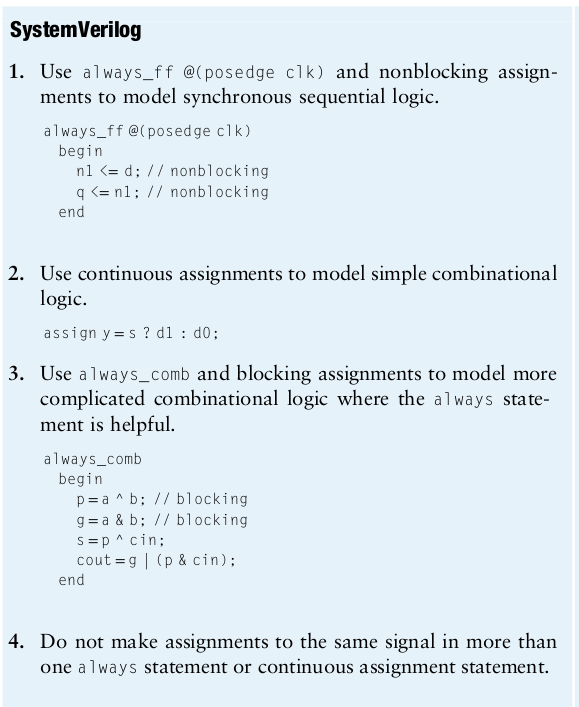
\includegraphics[width=0.4\linewidth]{./blocking-vs-non-blocking-assignment.png}

\begin{question}
  What's the deal with \lstinline[style=verilog-style]{initial} block?
\end{question}
You should only use \lstinline[style=verilog-style]{initial} block for
simulation. It is a non-synthesizable block, so it will not be converted into a
circuit. Instead, use a reset signal and an \lstinline[style=verilog-style]{if (reset)}
block to initialize your states.

\end{document}